\chapter{Thematische Vorbemerkung} \label{sec:thema}

Im ersten Teil dieses Kapitels werden zunächst einmal die Grundlagen zu Augmented Reality beschrieben, wie diese Technologie einzuordnen ist, welche technischen Anforderungen ein Augmented Reality System hat und wo typische Einsatzszenarien liegen. Außerdem wird hier auf den aktuellen Stand der Forschung bezüglich der Bestimmung von Überdeckungen in einem Augmented Reality System eingegangen. Hiernach wird näher auf Googles Project Tango eingegangen, welche Konzepte angewendet werden und wie diese Technologie im Bereich Augmented Reality einzuordnen ist. \\


\section{Augmented Reality}

Augmented Reality (AR) ist eine Klasse aus dem Realitäts-Virtualitäts-Kontinuum von \cite{milgram1995augmented}, welches in Abbildung \ref{fig:virtual-continuum} abgebildet ist. Diese Klasse beschreibt die Darstellungen von realen und virtuellen Informationen in einer Repräsentationsform, wobei hier reale und virtuelle Objekte in einer realen Umgebung kombiniert dargestellt werden können. Diese virtuellen Objekte sind in der realen Umgebung idealerweise fest lokalisiert und fügen sich somit in das reale Erscheinungsbild ein. Typischerweise sind AR Anwendungen interaktiv, und stellen die virtuellen Objekte in Echtzeit und dreidimensional in der realen Welt dar. Für die Definition von AR Anwendungen gibt es zudem keine Limitierung für die Darstellungstechnologie, wie zum Beispiel das Project Tango Tablett oder einem Head-Mounted-Display. AR beschränkt sich zudem nicht auf den angesprochenen Sinn - so sind zum Beispiel AR Anwendungen mit visueller, taktiler oder sogar olfaktorischer Umsetzung möglich.

\begin{figure}
  \centering
	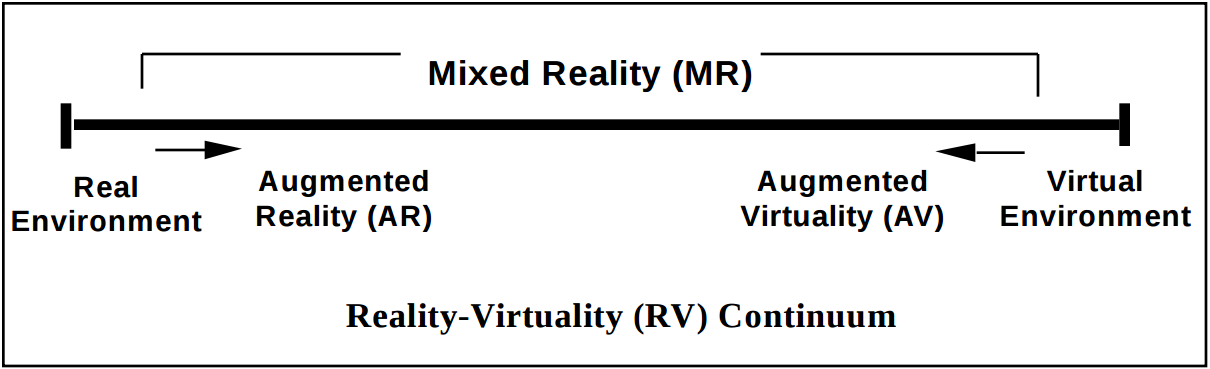
\includegraphics[width=0.85\textwidth]{content/images/theory/virtual-continuum.png} 
  \caption{Vereinfachte Darstellung des Realitäts-Virtualitäts-Kontinuum von \citet*{milgram1995augmented}}
  \label{fig:virtual-continuum}
\end{figure}


Virtuel Reality (VR) oder auch Virtual Environment hingegen kapselt sich von der realen Umgebung ab und bietet Interaktionen in reinen virtuellen Umgebungen. Diese rein virtuelle Darstellung konnte sich im Gegensatz zu Augmented Reality deutlich schneller Entwickeln, da die technologischen Anforderungen an AR deutlich höher sind. \citep{van2010survey}

\subsection{Technische Anforderungen}

Dieser Abschnitt widmet sich den technischen Anforderungen an Augmented Reality, indem die potentiellen Display Technologien beschrieben werden, mögliche Trackingverfahren zur Ermittlung der Betrachtungsposition erläutern werden und auch die Systeme behandelt werden, mit denen ein Nutzer mit den virtuellen Darstellungen interagieren kann.

\subsubsection{Display Technologie}

Der erste wichtige Teil der technologischen Anforderungen an AR sind visuelle Anzeigen (visual displays), die neben der Möglichkeit eines dreidimensionalen Renderings, welches hier aus der Virtual Reality vorausgesetzt werden soll, weitere Charakteristika mit sich bringen. Nach \citet{van2010survey} lassen sich diese Technologien zunächst in je drei Arten der Darstellung und Positionierung unterteilen.

Die einfachste und günstigste Art der visuellen Darstellung in AR ist \enquote{video see-through}, wodurch die reale Umgebung durch eine Video Aufnahme ersetzt wird und die virtuellen Objekte digital in die Video Aufnahme gerendert werden. Das bietet die Möglichkeit Objekte aus der realen Umgebung zu entfernen oder zu ändern oder, anhand der Luminanz Information vom Video, das Rendering der virtuellen Objekte entsprechend an die Realität anzupassen. Anwendung findet diese Technologie typischerweise in Tablets, Smartphones oder Head-Mounted-Displays.

Die nächste Möglichkeit zur Darstellung ist \enquote{optical see-through}. Hier werden die virtuellen Objekte durch transparente Spiegel in das Sichtfeld des Betrachters gebracht. Anders als bei \enquote{video see-throught} bleibt die reale Auflösung für die visuelle Aufnahme des Betrachtes gleich und es können zudem nur Latenzprobleme bei dem Rendering der virtuellen Objekte und nicht bei der Darstellung der realen Umgebung auftreten. Auf der anderen Seite besteht bei dieser Technologie das Problem, dass die Darstellung von virtuellen Objekten nicht kräftig genug ist, um die reale Umgebung auf Grund von der transparenten Darstellungsoberfläche komplett auszublenden. Typische Geräte dieser Technologie sind Headmounted Displays wie Google Glass\footnote{\url{https://developers.google.com/glass/} (23.02.2016)} oder stationäre Geräte wie der HoloDesk\footnote{\url{http://research.microsoft.com/en-us/projects/holodesk/} (23.02.2016)}.

Die dritte Möglichkeit ist die projizierte Darstellung, in der die Augmented Reality Überlagerung auf die realen Objekte projiziert werden. Diese Darstellung ermöglicht die Abdeckung vom gesamten Sichtfeld des Betrachters, benötigt aber eine entsprechende Kalibrierung oder eine Strukturwahrnehmung bei Umgebungsänderungen.

Neben der Art der Darstellung können die Display Technologien laut \citet{azuma2001recent} anhand Ihrer Positionierung klassifiziert werden. Man unterscheidet zwischen am Kopf befestigten Displays (head-mounted), tragbaren Displays (hand-held) und räumlich positionierten Displays. Zu jeder dieser Displayarten gibt es wiederum unterschiedliche technische Umsetzungen mit ihren spezifischen Vor- und Nachteilen bezüglich ihrer Anwendungsszenarien.

\subsubsection{Tracking Technologien}

Um eine virtuelle Projektion im realen Raum auf nicht stationären Displaytechnologien zu realisieren muss die Position und gegebenenfalls relative Positionsänderung des Displays bestimmt werden, auch \enquote{augmented reality registration} genannt. Man spricht dabei üblichweise von den \enquote{six degrees of freedom (6DOF)}, der Position im Raum (x, y, z) und der Orientierung (yaw, pitch, roll). 

Frühe Techniken für die Registrierung benötigten üblicher Weise eine speziell vorbereitete Räumlichkeit, denn sie basierten auf mechanischen, magnetischen oder Ultraschall Sensoren um die Position zu bestimmen. Diese Sensoren sind zwar immer noch im Einsatz und bilden auch den Grundstein für die AR und VR Forschung, sind aber praktisch gesehen zu komplex und aufwändig für die meisten Anwendungsfälle. \citep{van2010survey} 

Für ein grobes Positions-Tracking, vor allem auch außerhalb von Gebäuden wird GPS genutzt. Für großräumige Anwendung ist GPS, mit einer Varianz von 10-15 Metern und in Kombination mit einem Kompass, durchaus praktikabel. Als Beispiel reicht diese Genauigkeit aus, um sichtbare Flugzeuge oder Sterne visuell aufzubereiten. Innerhalb von Gebäuden basiert die grobe Positionierung laut \citet{van2010survey} oft auf verfügbaren Wifi Access Points oder RFID Markern. \citet{lamarca2005place} demonstrieren hierzu auch die Möglichkeit diese Idee für grobe Lokalisation außerhalb von Gebäuden einzusetzen.

Optische Tracking Verfahren, basierend auf Bildverarbeitung, bieten laut \citet{van2010survey} deutlich genauere Resultate als die zuvor beschriebenen Verfahren. Es gibt hier viele verschiedene sensorische Ansätze ein optisches Tracking zu realisieren. Frühe verfahren, wie die von \citet{dunston2008identification} oder \citet{narzt2006augmented}, nutzten Passmarker (fiducial marker) oder Licht emittierende LEDs in einem vordefinierten Modell, um zwischen aufgenommenen Bildern die Marker oder LEDs zu detektieren und zusammengehörige zwischen den Bildern zu finden, um daraus eine Kameratransformation zu berechnen. Neue Verfahren ohne Marker, wie das sogenannte \enquote{visual odometry} von \citet{nister2004visual}, nutzen Techniken zur Feature Detection und Matching um Referenzen und Bewegungen zwischen aufgenommenen Bildern zu bestimmen.

Viele kommerzielle und erfolgreiche Tracking Verfahren beruhen jedoch auf hybride Ansätze, in denen die Informationen mehrerer Sensoren kombiniert werden, um potentielle Messfehler eines Sensors oder einer Methodik auszuschließen. So werden zum Beispiel Neigungssensor, Kompass und Gyroskop mit einem optischen Verfahren kombiniert, um ein Tracking der sechs Freiheitsgrade zu optimieren. Diese Erweiterung des optischen Verfahrens wird auch \enquote{visual-inertial odometry} genannt. \citep{van2010survey}

\citet{azuma2001recent} erwähnt an dieser Stelle auch die Kalibrierung der Sensoren, die für ein präzises Registrieren nötig ist. So müssen zum Beispiel die Linseneigenschaften der Kamera für optisches Tracking bekannt sein, damit die Verfahren mit Krümmungen, Verzerrungen und den perspektivischen Eigenschaften der Kamera umgehen können. Diese Informationen sind auch bei video see-through Displays für ein korrektes Projizieren der 3D Objekte wichtig. Zudem wird erwähnt, dass man Messfehlern oder Drifts der Position zum Beispiel mit der Zunahme von Gyroscop Informationen entgegenwirken kann, indem man Ereignisse wie einen Schritt des Nutzers einfließen lässt. \citep{azuma2001recent} 

\subsubsection{Interaktions Technologien} \label{sec:ar-interaction}

Neben den Display und Tracking Technologien ist es notwendig dem Nutzer andere Interaktionsmöglichkeiten anzubieten, da in der Regel das klassische zweidimensionale WIMP Paradigma (Windows, Icons, Menus and Pointer) im dreidimensionalen Kontext von AR keine ausreichende Gebrauchstauglichkeit bietet. Dennoch müssen die Interaktionstechnologien in Augmented Reality die üblichen Interaktionen wie aus WIMP unterstützen. Dazu gehören zum Beispiel das Auswählen, Positionieren und Drehen von virtuellen Objekten, das Zeichnen von Pfaden oder Flugbahnen, sowie die Eingabe von Quantitativen Werten oder Texten. \citep{van2010survey} 

Frühe Augmented Realilty Systeme nutzen einfache Trackballs, Trackpads, Touchscreens oder Gyroscopmäuse für eine zweidimensionale Interaktion mit dem System. Später wurden dreidimensionale Equivalente eingeführt, wie 3D Mäuse oder Stifte, die eine dreidimensionale Interaktion ermöglichen. Diese Greifbaren Schnittstellen werden auch TUIs genannt (Tangible User Interface) und ermöglichen eine unidirektionale Interaktion mit dem System. Zudem wurden auch TUIs mit haptischen Feedback eingeführt, wie zum Beispiel die 3D Maus PHANTOM. \citep{van2010survey} 

Eine weitere Art der TUIs sind laut \citet{azuma2001recent} Gegenstände, mit denen der Nutzer natürlich interagieren kann und die vom System optisch erfasst werden, um die Positionsänderung der Objekte anhand von Markern oder anderen optischen Merkmalen zu bestimmen. Somit kann ein Nutzer, zum Beispiel, für die virtuelle Einrichtung eines Raums, die Möbel mit Hilfe eines echten Gegenstands im Raum verschieben. 

Nicht taktile Systeme verwenden meist optische Aufnahmen, um Gesten der Hände, des gesamten Körpers oder die Blickrichtung des Nutzers erkennen zu können. Für die Realisierung werden dazu Kameras am Körper oder im Raum verwendet. Außerdem ist es möglich Spracherkennung in die Interaktion mit einfließen zu lassen, um eine möglichst authentische Interaktion zu bieten. Wie auch bei den Tracking Technologien existieren hierbei Hybride Systeme, die verschiedene Interaktions Technologien kombinieren. \citep{van2010survey} 

\subsection{Anwendungsbereiche}

Über die Jahre habe Wissenschaftler immer mehr Bereiche identifiziert, die von der Anwendung von Augmented Reality profitieren können. \citet{van2010survey} nennt dazu als Erstes Einsatzgebiet die persönliche Assistenz, in der AR Systeme eingesetzt werden können, um zum Beispiel mit Hilfe von Brillen (zum Beispiel der Google Glass) Namen der sichtbaren Personen anzuzeigen, die Navigation in unbekannten Regionen einzublenden oder beim Sightseeing Kontext relevante Informationen im Sichtfeld anzuzeigen. 

Neben der persönlichen Assistenz können auch Anwendungen in der Industrie laut \citet{van2010survey} von AR profitieren. Es lassen sich zum Beispiel virtuelle Designumgebungen umsetzten, die es ermöglichen ein Auto in Lebensgröße zu Gestalten. Auch bei der Fertigung und Konstruktion können den Arbeitern unterstützende Informationen angezeigt werden. So werden zum Beispiel zu erledigende Schweißstellen hervorgehoben oder der Plan zur Konstruktion entsprechend eingeblendet. Oder für die Instandhaltung komplexer Maschinen kann ein AR System dem Nutzer eine Art Röntgenblick Hinweise auf potentielle Schwachstellen liefern. Auch in der Rüstungsindustrie existieren Anwendungsgebiete für Augmented Reality Systeme. So können zum Beispiel Gefechte für eine Kampfausbildung besser simuliert werden. \citep{azuma2001recent} 

Für Anwendungsbereiche in der Medizin ist ein sehr genaues Tracking der Freiheitsgrade erforderlich, da AR in der Chirurgie und Behandlung von Patienten Anwendung findet. Erstellte Röntgenbilder oder Ultraschallbilder können hierdurch, anstatt auf einem separaten Monitor, direkt auf die entsprechende Körperstelle projiziert werden, wodurch gegebenenfalls eine genauere Untersuchung oder Behandlung möglich ist. \citep{van2010survey} 

Augmented Reality wird auch im Entertainment Sektor eingesetzt. Videoübertragungen von Sportereignissen werden heutzutage oft durch zusätzliche Informationen angereichert. So erhalten zum Beispiel American Football Spiele dynamische Spielfeld Begrenzungen. Auch die Werbeeinblendungen am Rand des Spielfelds können entsprechend dem Gebiet der Ausstrahlung ausgetauscht werden. \citep{azuma2001recent} 

Ein weiteres großes Anwendungsgebiet für Augmented Reality sind laut \citet{azuma2001recent} Computerspiele, in denen es möglich ist, in einer beliebigen Umgebung Objekte eines Spiels im Raum zu platzieren und mit Ihnen entsprechend zu interagieren. Die natürlichere Interaktion, gegenüber herkömmlichen Spielplattformen, und die Nutzung in einer persönlichen Spielumgebung führt zu einem intensiveren Spielerlebnis. 

In der Bildung für Schulen oder Museen ist es auch mögliche AR Systeme einzusetzen. Zur Vermittlung von geometrischen oder mathematischen Grundlagen gibt es die Möglichkeit der kollaborativen und interaktiven Visualisierung von Körpern, an denen etwa Parameter manipuliert werden, um danach Ihre Eigenschaften besser beobachten und nachvollziehen zu können. \citep{van2010survey} 

\subsection{Einschränkungen und Probleme}

Die frühen Augmented Reality Systeme sind auf Grund ihrer Größe sehr unhandlich und mobil daher nur mit großem Aufwand anwendbar. Durch die Verfügbarkeit mobiler und performanter Endgeräte ist ein mobiler Einsatz wiederum ermöglicht worden. Jedoch besitzen die aktuellen Geräte wie Smartphones oder Tabletts nicht die entsprechende Sensorik für ein präzises Tracking der sechs Freiheitsgrade. \citet{van2010survey} weisen zudem darauf hin, dass die Registrierung der Tiefe für die Anwendung von Überdeckungen oder korrekter Positionierung bei einer Interaktion ein komplexes Problem sei. Wie in Kapitel \ref{sec:theory_project_tango} zu finden geht Project Tango dieses Problem der Sensorik entsprechend an und versucht Schnittstellen zu bieten, um sowohl das Tracking zu ermöglichen und Tiefeninformationen über die aktuelle Szene zu liefern. 

Eine weitere erwähnenswerte Problematik ist neben der sensorischen Themen von Augmented Reality die Herangehensweise zur Gestaltung der Nutzeroberflächen für AR. Denn die UI Konzeption gestaltet sich, laut \citet{azuma2001recent}, als schwierig. Die Anreicherungen durch Augmented Reality führt schnell dazu, dass das Sichtfeld überladen wirkt. Jedoch soll dem Nutzer immer die Informationen zur Verfügung gestellt werden, die gegebenenfalls kontextsensitiv und relevant sind. Diese Angesprochenen Faktoren führen aktuell bei Augmented Reality Anwendungsgebieten noch zu einer geringen Akzeptanz der Endverbraucher.

\subsection{Realisierung von Augmented Reality Über\-deckungen} \label{sec:ar-occlusion}

Es gibt einige Verfahren und Ansätze, um eine Überlagerung in Augmented Reality Szene zu realisieren. \citet{wloka1995resolving} bilden hierfur den Grundstein für die verschiedenen existierenden Methoden. Sie stellen in Ihrer Arbeit ein Verfahren vor, welches mit Bildern aus einer Stereo Kamera ein Stereomatching durchführt und dadurch ein Tiefenbild generiert. Dieses Tiefenbild führt in dem Renderingprozess mit Hilfe des Z-Buffer Algorithmus (beschrieben in Kapitel \ref{sec:z-buffer}) zum Ausschluss von Teilen der virtuellen Objekte, die von realen Objekten überlagert werden. Das Ergebnis des Stereomatchings ist in ihrer Arbeit mit gewissen Ungenauigkeiten behaftet und generiert unerwünschte Lücken in der Projektion des virtuellen Objekts. Arbeiten wie von \citet{seo2013direct}, mit neuen Tiefensensoren wie der Microsoft Kinect\footnote{Microsoft Kinect - https://dev.windows.com/en-us/kinect (04.03.16)}, erhalten durch den selben Mechanismus deutlich bessere Ergebnisse. 

Die Arbeit von \citet{breen1996interactive} nahmen diesen Ansatz von \citet{wloka1995resolving} auf und stellten die Idee vor, neben einer deutlich genaueren Überdeckung auch eine Interaktion mit realen Objekten zu realisieren. Hierfür werden virtuelle Modelle der realen Objekte in der Szene passend an der echten Umgebung und der Position der realen Objekte ausgerichtet. Dieses Vorgehen setzt jedoch voraus, dass die entsprechenden virtuellen Modelle für die realen Objekte bereits vorliegen. Nach dieser Ausrichtung wird die Tiefe der virtuellen Objekte gewonnen, um daraus, mit dem Verfahren von \citet{wloka1995resolving}, eine Überlagerung durch den Ausschluss der weiteren virtuellen Objekten der Szene zu bewirken. 

Neben den Modell basierten Verfahren existieren auch Kanten basierte Verfahren, wie das von \citet{berger1997resolving}, in dem Objektkanten auf optischer Basis mit Filtern ermittelt werden. Diese Kanten werden über mehrere Bilder verfolgt, um die Tiefeninformation der Kanten durch Epipolargeometrie und Heuristiken zu bestimmen. \citet{berger1997resolving} gewinnt darauf folgend  eine Tiefenmaske, indem er annimmt, dass Konturen, die unter einer gewissen Distanz von einander entfernt sind, zu einem Objekt gehören. \citet{klein2004sensor} erreichen mit einer, auf mobiler Hardware umgesetzten Umgebung, mit diesem Verfahren, sehr überzeugende Ergebnisse in einer vordefinierten Umgebung. Zwar verspricht dieses Vorgehen eine Kanten genaue Überdeckung virtueller Objekte, führt aber bei komplexeren Szenen, in denen die Kanten nicht mehr erfolgreich verfolgt werden oder nicht zu einem Objekt zugeordnet werden können, zu Fehldarstellungen. Außerdem werden Ausbreitungen innerhalb des Objekts, welche nicht als Kante erkannt werden können, nicht berücksichtigt.

Die letzte Variante wurde von \citet{breen1996interactive} bereits erwähnt, ist die Ermittlung der Überdeckung durch eine Rekonstruktion der Szene. Dieser Ansatz verschiebt durch das Verfahren von \citet{wloka1995resolving} die Problemstellung der AR Überdeckung in den Bereich der Echtzeit Rekonstruktionsproblematik. Bekannte Verfahren hierfür sind zum Beispiel KiniectFusion von \citet{newcombe2011kinectfusion} oder die Echtzeit Rekonstruktion von \citep{niessner2013real}. Diese sehr komplexen Verfahren sind meist auf der Grafikhardware von Desktopsystemen umgesetzt und generieren eine detaillierte Rekonstruktionen aus den Tiefeninformationen in Echtzeit. Diese Rekonstruktionen können laut \citet{newcombe2011kinectfusion} für eine Echtzeit Überdeckung in Augmented Reality Systemen dienen. Vorteilhaft bei einer Rekonstuktions basierter Überdeckung ist zudem, dass auch Interaktionen mit echten Objekten, wie bei \citet{breen1996interactive}, erfolgreich umgesetzt werden können.





\section{Project Tango} \label{sec:theory_project_tango}

Project Tango ist eine Technologie Plattform für Android Tablets und Smartphones von Google’s Advanced Technology and Projects Group (ATAP). Das Ziel dieser Plattform ist es, Motion Tracking (Positionierung), Depth Perception (Tiefeninformation/Pointcloud) und Area Learning (Lokalisierung) auf mobile Endgeräte zu bringen, um verschiedenste Anwendungs-Szenarien abzudecken. Typische Szenarien sind Indoor Navigation, Virtual Reality Anwendungen, Vermessungs- und Rekonstruktions\-software und Augmented Reality Anwendungen.

Das System ermöglicht in erster Linie ein Tracking von Positionsänderungen des Geräts im Raum und bietet somit eine genaue relative Lokalisierung. Mit Hilfe dieser Lokalisierung und der Hinzunahme von visuellen Merkmalen im Raum ist das Gerät in der Lage, seine Umgebung kennenzulernen und gegebenenfalls die Lokalisierung zu korrigieren oder aber diese in einer bereits erlernten Umgebung zu bestimmen. Zusätzlich bietet Project Tango die Möglichkeit, mit Hilfe eines Tiefensensors, eine Pointcloud der Tiefeninformation pro Bildausschnitt zu ermitteln, um Anwendungen auch räumliche Informationen bereitzustellen.  \citep{Proje19:online} 

\subsection{Geräte und Hardware}

Da das Project Tango zum Zeitpunkt der Verfassung dieser Thesis noch unter Entwicklung steht, gibt es von Google nur erste Entwickler Prototypen. Das erste Gerät \enquote{Peanut Phone} im Smartphone Format, welches in Abbildung \ref{fig:tango-device} rechts unten zu erkennen ist, wurde Anfang 2014 veröffentlicht und ein halbes Jahr später bereits durch eine neue Generation, dem \enquote{Yellowstone Tablet} ersetzt. Dieses 7\dq Tablet, zu sehen rechts oben im Bild \ref{fig:tango-device}, verfügt, wie in der Abbildung links zu erkennen, über einen Infrarot Laser Projektor, eine Fisheye Kamera und eine normale 4 Megapixel Kamera auf der Rückseite. Zudem sind, wie in aktuellen Smartphones und Tablets üblich, ein Beschleunigungssensor, Umgebungslichtsensor, Barometer, Kompass, GPS und ein Gyroskop verbaut. Das Gerät wird von einem NVIDIA Tegra K1 Prozessor betrieben und verfügt über 4GB Arbeitsspeicher. \citep{Proje19:online} Mit diesem Gerät wurden die später beschriebenen Techniken umgesetzt und evaluiert. 

\begin{figure}[h]
  \centering
	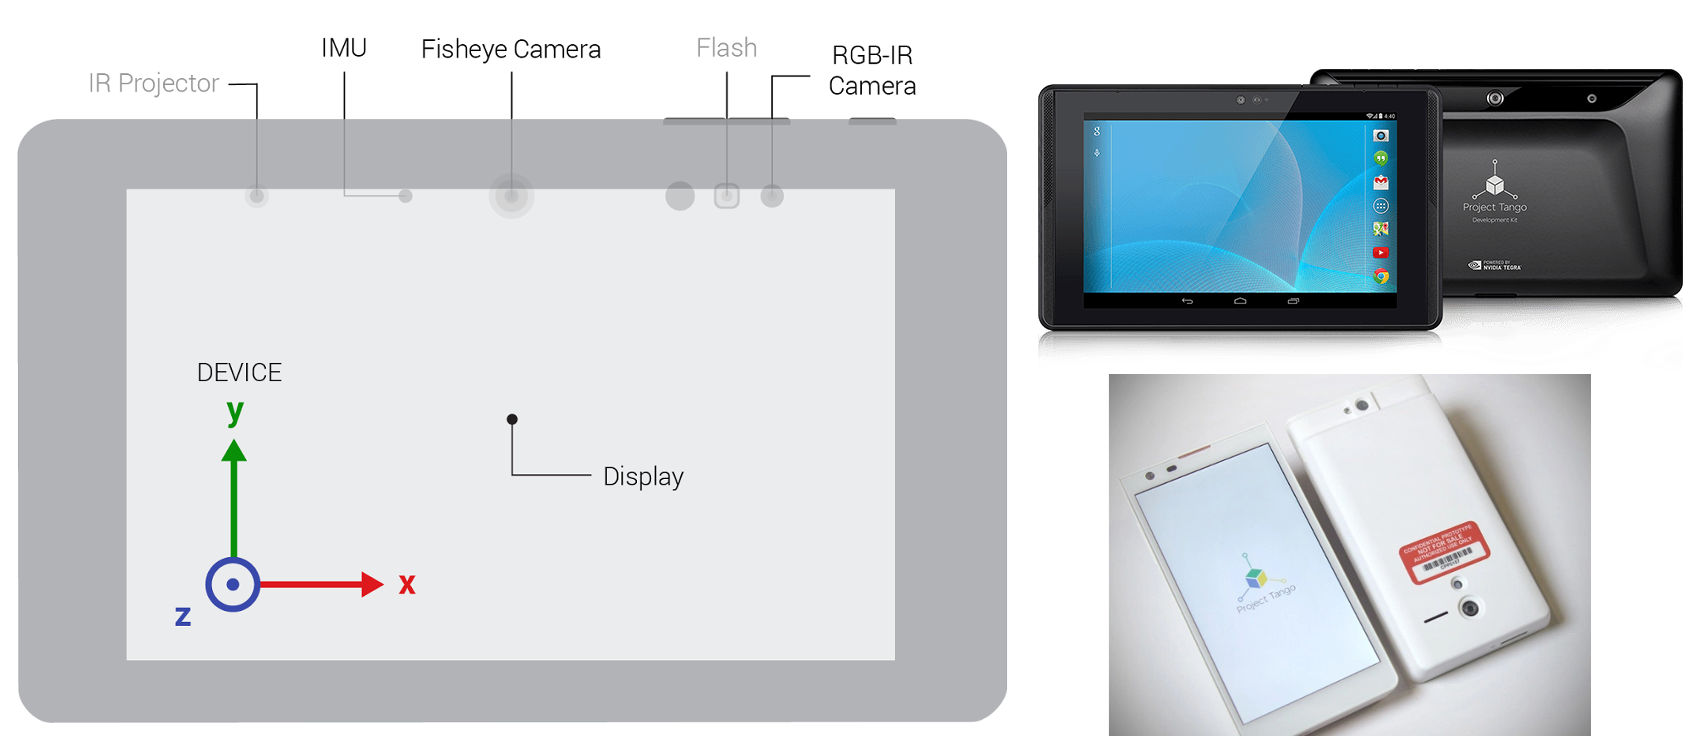
\includegraphics[width=1.0\textwidth]{content/images/theory/tango-device.png} 
  \caption{Links: schematischer Aufbau der Google Project Tango Hardware. Rechts: Das aktuelle Entwickler Gerät im Tablet Format (oben) und das alte Entwickler Gerät im Smartphone Format (unten). Übernommen von \citet{GoogleDevelopers:online}}
  \label{fig:tango-device}
\end{figure}

\subsection{Konzepte und Schnittstellen}

Generell betrachtet ist das Project Tango eine Plattform, die Computer Vision nutzt, um dem Gerät die Möglichkeit zu bieten seine relative Positionierung in der umgebenden Szene in Echtzeit zu bestimmen. Auf den Geräten kommt Googles Android Betriebsystem zum Einsatz, weshalb zu beachten ist, dass es sich bei der Plattform nur bedingt um eine Echtzeitumgebung handelt. Das liegt daran, dass der Linux Kernel keine Garantien für die zeitlich präzise Ausführung von Instruktionen auf Grund von Scheduling geben kann. Google weist daher darauf hin, dass das System als \enquote{soft-realtime} betrachtet werden sollte. Daher sollten Messergebnisse verschiedener Sensoren unter Berücksichtigung ihrer Aufnahmezeitpunkte verwendet werden. \citep{GoogleDevelopersConcepts:online} 

\subsubsection{Motion Tracking}

Um die relative Bewegung vom Start des Project Tango Systems bestimmen zu können, nutzt es \enquote{visual-inertial odometry}. \citep{GoogleDevelopersConcepts:online}
Dabei handelt es sich um eine erweiterte Variante von Visual Odometry. 
Das von \citet{nister2004visual} veröffentlichte Verfahren Visual Odometry ist in der Lage aus einfachen Videoinhalten in Echtzeit die Bewegung der Kamera zu bestimmen. 
Hierzu werden zunächst übergreifende Features, zum Beispiel Punkte aus der FAST Kantenerkennung von \citet{trajkovic1998fast}, aus mehreren Bildern bestimmt. Um daraus eine Transformation zwischen den Bildern ermitteln zu können, wird der 5-point Algorithmus von \citet{nister2004efficient} angewendet. Dieser Algorithmus ist in der Lage das Problem zu lösen, eine relative Transformation zwischen zwei Bildern mit gegebenen 5 Punktübereinstimmungen zu ermitteln. Außerdem wird erwähnt, dass mit Hilfe des Schätzverfahrens RANSAC (beschrieben in Absatz \ref{sec:ransac}) bei einer Überbestimmung des Modells, ein potentieller Fehler deutlich minimiert werden kann. 

Project Tango lässt an dieser Stelle die internen Sensoren zur Rotation, Orientierung und Bewegung mit in die Bestimmung der Kameratransformation einfließen, um so ein präziseres Ergebnis erzielen zu können. Außerdem wird versucht mit Hilfe des Kalman Filters, nach dem gleichnamigen Autor \citet{kalman1960new}, die Fehler der Sensoren bei dieser Echtzeitmessung zu reduzieren. Über eine längere Messzeit oder eine größere Entfernung vom Ursprung kann es jedoch zu kleinen Abweichungen kommen. Außerdem existiert zum aktuellen Zeitpunkt noch ein \enquote{Drift} Problem\footnote{Das Drift Problem tritt auf, wenn zu wenige übereinstimmende Punkte im Raum zwischen den Bildaufnahmen der Fisheye Kamera gefunden werden. Das führt in der Regel zu relativen Bewegungen der virtuellen Kamera obwohl keine reale Bewegung statt findet.}, was zu großen Messfehlern führen kann. Es wird jedoch versucht diese Probleme mit dem Konzept \enquote{Area Learning}, beschrieben in Kapitel \ref{subsec:area-learning}, zu lösen. \citep{GoogleDevelopersConcepts:online}

Wie genau das Verfahren aussieht, welche Techniken zur Feature Detection oder Feature Matching genutzt werden und welche Features hierfür erkannt werden, ist nicht bekannt. \citet{Klingensmith_2015_7924}, als Mitglieder von Googles Advanced Technologies and Projects Abteilung ATAP, erwähnen jedoch, dass nähere Informationen über das Verfahren von \citet{kottas2013consistency} und \citet{mourikis2007multi} beschrieben werden. Sie erläutern in ihren Arbeiten, welche Mechanismen eingesetzt werden können, um eine Migration aller Sensorinformationen für ein zuverlässiges hybrides optisches Tracking zu realisieren.

\subsubsection{Depth Perception}

Zur Tiefenmessung ist die Project Tango Hardware mit einem kalibrierten Infrarot Laserprojektor ausgestattet. Dieser streut Infrarot Punkte mit einer Auflösung von 320 x 180 Punkten in den Raum, um mithilfe von Aufnahmen der RGB Kamera eine Punktewolke der Tiefeninformation zu bestimmen. Aufgrund einer ausgewogenen Konfiguration zwischen Messbereich, Messfehlern und dem Energieverbrauch, liegt der Messbereich der Sensorkombination, laut \citet{GoogleDevelopersConcepts:online}, zwischen einem halben und vier Metern. 

Dadurch, dass diese Technologie auf der Aufnahme von projiziertem Infrarotlicht basiert, ist ein Einsatz der Tiefenmessung außerhalb geschlossener Räume nicht möglich \citep{GoogleDevelopersConcepts:online}. Außerdem entstehen Messfehler durch reflektierende, lichtabsorbierende oder zu komplex strukturierte Oberflächen, wie zum Beispiel Metalle, LCD Monitore oder Hochflor Teppiche. 

Die zuvor erwähnten Punktewolken werden in dem eigens definierten XYZij Format von der Entwicklungsschnittstelle zurückgegeben. Dabei wird jeder Punkt mit den \(X\), \(Y\) und \(Z\) Koordinaten im Weltkoordinatensystem und den beiden Indizes \(i \) und \(j \) für die Spalte und Zeile der projizierten Punkte auf der Bildebene angegeben \citep{GoogleDevelopersConcepts:online}. Man spricht dabei von einer organisierten Punktewolke, da durch die \(i\) und \(j\) Koordinaten die direkten Nachbarn, ausgehend von dem Aufnahmeblickwinkel, eines Punktes bestimmt werden können. Hieraus ist es möglich Tiefenbilder, die sogenannten \enquote{Depth Maps}, zu bestimmen, für die es viele verschiedene Computer Vision Verfahren zur Bestimmung von Objekten, Strukturen und Fluchtpunkten gibt. Die Schnittstellen liefern jedoch, laut \citet{GoogleDevelopersKnownIssues:online}, zum aktuellen Entwicklungsstand die beschriebenen Informationen über die Spalten \(i\) und Zeilen \(j\) noch nicht.

\citet{GoogleDevelopersConcepts:online} weist darauf hin, dass das Generieren von polygonbasierten Rekonstruktionen noch nicht in den Schnittstellen enthalten ist. Es gibt jedoch freie Dritt-Bibliotheken und -Systeme, wie das Robot Operating System\footnote{Robot Operating System - \url{http://ros.org/} (23.02.2016)} oder die Point Cloud Library\footnote{Pointcloud Library - \url{http://pointclouds.org/} (23.02.2016)}, die für eine weitere Verarbeitung genutzt werden können.

\subsubsection{Area Learning} \label{subsec:area-learning}

Area Learning bezeichnet den Prozess, in dem Project Tango Geräte in der Lage sind, durch visuelle Hinweise die umgebende Welt kennenzulernen und auf die Position des Gerätes zu schließen. 
Es ermöglicht somit eine Unterstützung für Motion Tracking und löst das Problem, das Gerät in einer bereits bekannten Umgebung zu lokalisieren, wie in Abbildung \ref{fig:area-learning} links zu erkennen ist.
Project Tango bietet außerdem die Möglichkeit diese visuellen Hinweise und ihre Position im Raum in sogenannten \enquote{Area Description Files} zu speichern und wiederzuverwenden. \citep{GoogleDevelopersConcepts:online}

\begin{figure}[h]
  \centering
	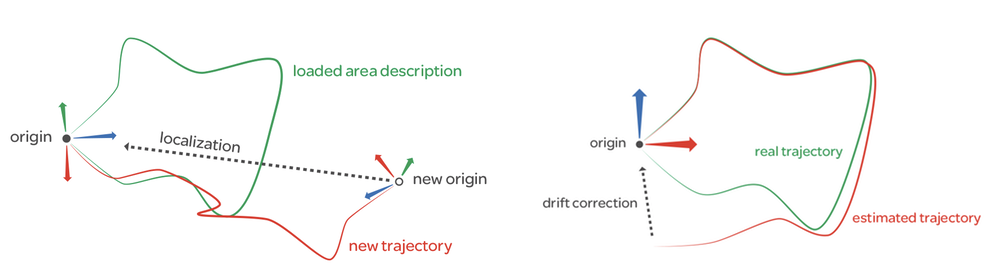
\includegraphics[width=1.0\textwidth]{content/images/theory/tango-area-learning.png} 
  \caption{Links: Lokalisierungsprozess durch Area Learning. Rechts: Korrektur von Motion Tracking anhand gelernter Merkmale. Übernommen von \citet{GoogleDevelopers:online}}
  \label{fig:area-learning}
\end{figure}

Wie bereits erwähnt entstehen bei Motion Tracking über eine längere Strecke Messfehler. 
Während diese Strecke mit einem Project Tango Gerät abgelaufen wird, ermittelt es fortlaufend die Position und den Pfad, den der Nutzer im Raum gegangen ist. 
Erkennt es während der Strecke visuelle Merkmale mittels Area Learning, wird der Pfad anhand der Positionen der Merkmale entsprechend angepasst. 
Project Tango unterscheidet hier zwischen zwei Manipulationen, \enquote{loop closures}, zur Zusammenführung des Pfads wenn ein Kreis gelaufen wurde, und \enquote{drift corrections}, um den erwähnten Drift-Effekt bei zu wenigen optischen Features im visual-inertial odometry zu korrigieren. 
Die drift correction ist in Abbildung \ref{fig:area-learning} rechts zu erkennen. \citep{GoogleDevelopersConcepts:online} 

Auch bei diesem Prozess werden die genauen Details nicht näher erläutert und es ist nicht bekannt, wie die Area Desciptions definiert sind oder was sie enthalten. \citet{GoogleDevelopersConcepts:online} weist jedoch darauf hin, dass, auch wenn die Area Desciptions Files keine direkten Bilder enthalten, es möglich sei, Rückschlüsse auf die gelernte Umgebung ziehen zu können. 

\subsection{Einordnung von Project Tango im Kontext der Augmented Reality} \label{sec:classification_project_tango}

Da sowohl die Grundlagen aus dem Bereich Augmented Reality als auch die technische Basis von Project Tango bekannt sind, kann die Project Tango Hardware bezüglich Augmented Reality näher eingeordnet werden. Bei der Hardware handelt es sich um ein hand-held Gerät, welches mit einer video see-through Display Technologie Augmented Reality Anwendungen ermöglicht. Hierfür kann wahlweise die normale RGB Kamera oder die Graustufen Fish-Eye Kamera verwendet werden. Für beide Kameras können die intrinsischen Kameraparameter ausgelesen werden, wodurch die Eigenschaften der realen Kamera durch die virtuelle Kamera übernommen werden können. Das führt zu einer parallax freien Überblendung und zu einer guten Tiefenwahrnehmung. 

Als Tracking Technologie wird hier eine hybride optische Variante angewendet. Dabei wird die Visual Odometry mit der Fish-Eye Kamera durch interne Sensoren für die Rotation, Orientierung und Bewegung kombiniert. Außerdem kann das Verfahren gegebenenfalls durch Googles Area Learning Mechanismen angereichert werden, um Messfehlern entgegenzuwirken. Die Eingabe erfolgt durch den Touchscreen des Tablets. Eine Interaktion mithilfe von optischer Gestenerkennung oder anhand der Tiefeninformationen ist zudem auch denkbar. 





